\documentclass{beamer}
\usefonttheme[onlymath]{serif}
% \usepackage[normalem]{ulem}
\usepackage{mathtools}
\usepackage{minted}
\usepackage{soul}
\usepackage{siunitx}

\title{Advent of Code -- Part 3: day 15}
\subtitle{A case study of algorithm development}
\author{Sigvald Marholm}
\institute[IFE]{Institute for Energy Technology\\Department of Computational Materials Processing}
\date{11.05.23}


\newenvironment<>{exenv}{\begin{altenv}#1%
    {\usebeamercolor[fg]{example text}}
    {}{\color{.}}{}\ignorespaces}{\ifhmode\unskip\fi\end{altenv}}
\newcommand<>{\ex}[1]{\begin{exenv}#2\relax#1\end{exenv}}

\begin{document}

    \begin{frame}
    \titlepage
    \end{frame}

    % \begin{frame}{Problem a}
    %    \begin{figure}
    %        \includegraphics[width=\textwidth]{example_input.png}
    %        \caption{Example input}
    %    \end{figure}
    % \end{frame}

    % \begin{frame}{Problem a}
    %    \begin{figure}
    %        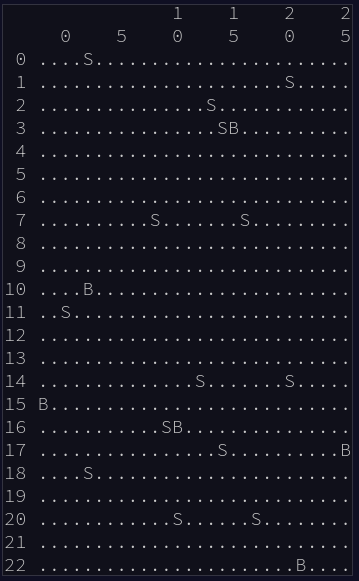
\includegraphics[width=0.4\textwidth]{example_arrangement.png}
    %        \caption{Example input}
    %    \end{figure}
    % \end{frame}

    % \begin{frame}{Problem a}
    %    \begin{figure}
    %        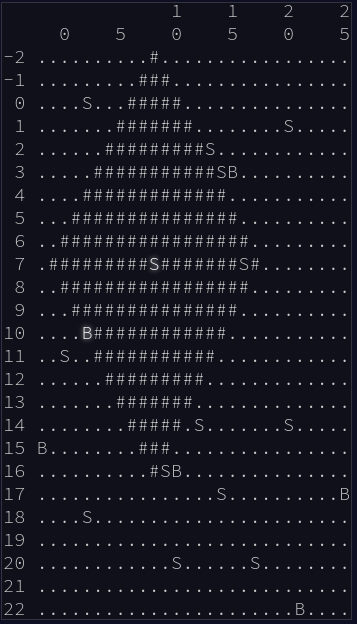
\includegraphics[width=0.4\textwidth]{example_coverage.png}
    %        \caption{Example input}
    %    \end{figure}
    % \end{frame}

    % GIVE DESCRIPTION OF PROBLEM WHILE LOOKING AT WEB PAGE

    \begin{frame}{The $p$-metric (in 2D)}
        \begin{columns}
            \begin{column}{0.49\textwidth}
                \[
                    d_p(\mathbf x, \mathbf x_s) = \sqrt[p]{|x-x_s|^p + |y-y_s|^p}
                \]
                {\small \mintinline{python}{np.linalg.norm([x-xs, y-ys], ord=p)}}

                \vspace*{3em}

                Manhattan metric ($p=1$):
                \[
                    d_1(\mathbf x, \mathbf x_s) = |x-x_s| + |y-y_s|
                \]
            \end{column}
            \begin{column}{0.49\textwidth}
                \begin{figure}
                    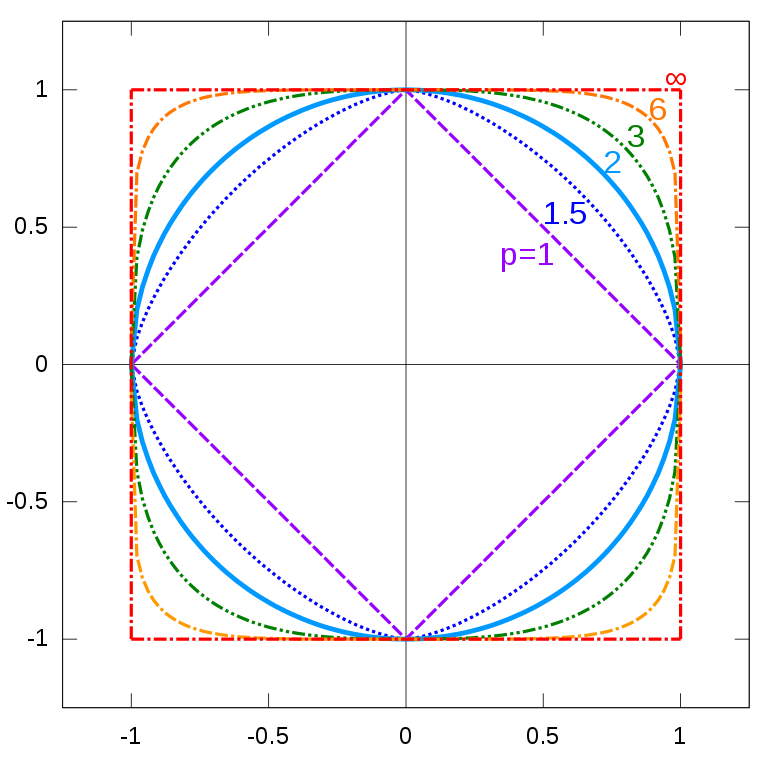
\includegraphics[width=0.8\textwidth]{p-norm.png}
                    \caption{A $p$-metric sphere. 

                    ~

                    \tiny Quartl, CC BY-SA 3.0, via Wikimedia Commons}
                \end{figure}
            \end{column}
        \end{columns}
    \end{frame}

    \begin{frame}[fragile]{Breaking down solution a}
        \framesubtitle{Parsing with regular expressions (and some functional programming)}
        \small
        % \begin{minted}[gobble=12]{python}
        \begin{minted}[gobble=12, fontsize=\scriptsize]{python}
            >>> line
            "Sensor at x=33790, y=3243415: closest beacon is at x=-355567, y=3900317"

            >>> re.findall("-?\d+", line) 
            ["33790", "3243415", "-355567", "3900317"]

            >>> map(int, re.findall("-?\d+", line))
            [33790, 3243415, -355567, 3900317]  # actually returns an iterable
        \end{minted}

        ~
        \pause

        Other \emph{regex} examples: \\
        \begin{minted}[gobble=12, fontsize=\scriptsize]{python}
            >>> re.search("\w+@\w+\.\w+", "Text with my@email.com inside").group()
            'my@email.com'

            >>> re.search("(\d{4})-(\d{2})-(\d{2})", "Today is 2023-05-13").groups()
            ('2023', '05', '13')
        \end{minted}
        % \mintinline{python}{"a"} matches ``a'' \\
        % \mintinline{python}{"[aA]"} matches ``a`` or ``A`` \\
        % \mintinline{python}{"[a-z]"} matches a lowercase letter \\
        % \mintinline{python}{"[a-z]+"} matches one or more lowercase letters \\
        % \mintinline{python}{"[a-z]*"} matches zero or more lowercase letters \\
        % \mintinline{python}{"[a-z]*"} matches zero or more lowercase letters \\
        % \mintinline{python}{"\d"} matches a digit \\
        % \mintinline{python}{"\d"} matches a digit \\
    \end{frame}

    \begin{frame}[fragile]{Breaking down solution a}
        \framesubtitle{Adding ranges of emptyness to a set}
        \begin{columns}
            \begin{column}{0.49\textwidth}
                Radius:
                \[
                    r = |x_b-x_s| + |y_b-y_s|
                \]
                \onslide<2->{
                    ``Rhombus-shaped'' ball:
                    \begin{align*}
                        r \leq |x-x_s| + |y-y_s|
                    \end{align*}
                }
                \onslide<3->{
                    Range for given $y$:
                    \[
                        |x-x_s| \leq \underbracket{r - |y-y_s|}_{\text{half-width}}
                    \]
                }
                \begin{uncoverenv}<4->
                    Sets have no order and unique elements: 
                    \begin{minted}[gobble=16, fontsize=\scriptsize]{python}
                        >>> {1, 3, 3, 2}
                        {1, 2, 3}
                    \end{minted}
                \end{uncoverenv}
            \end{column}
            \begin{column}{0.49\textwidth}
                \only<1-2>{
                    \begin{figure}
                        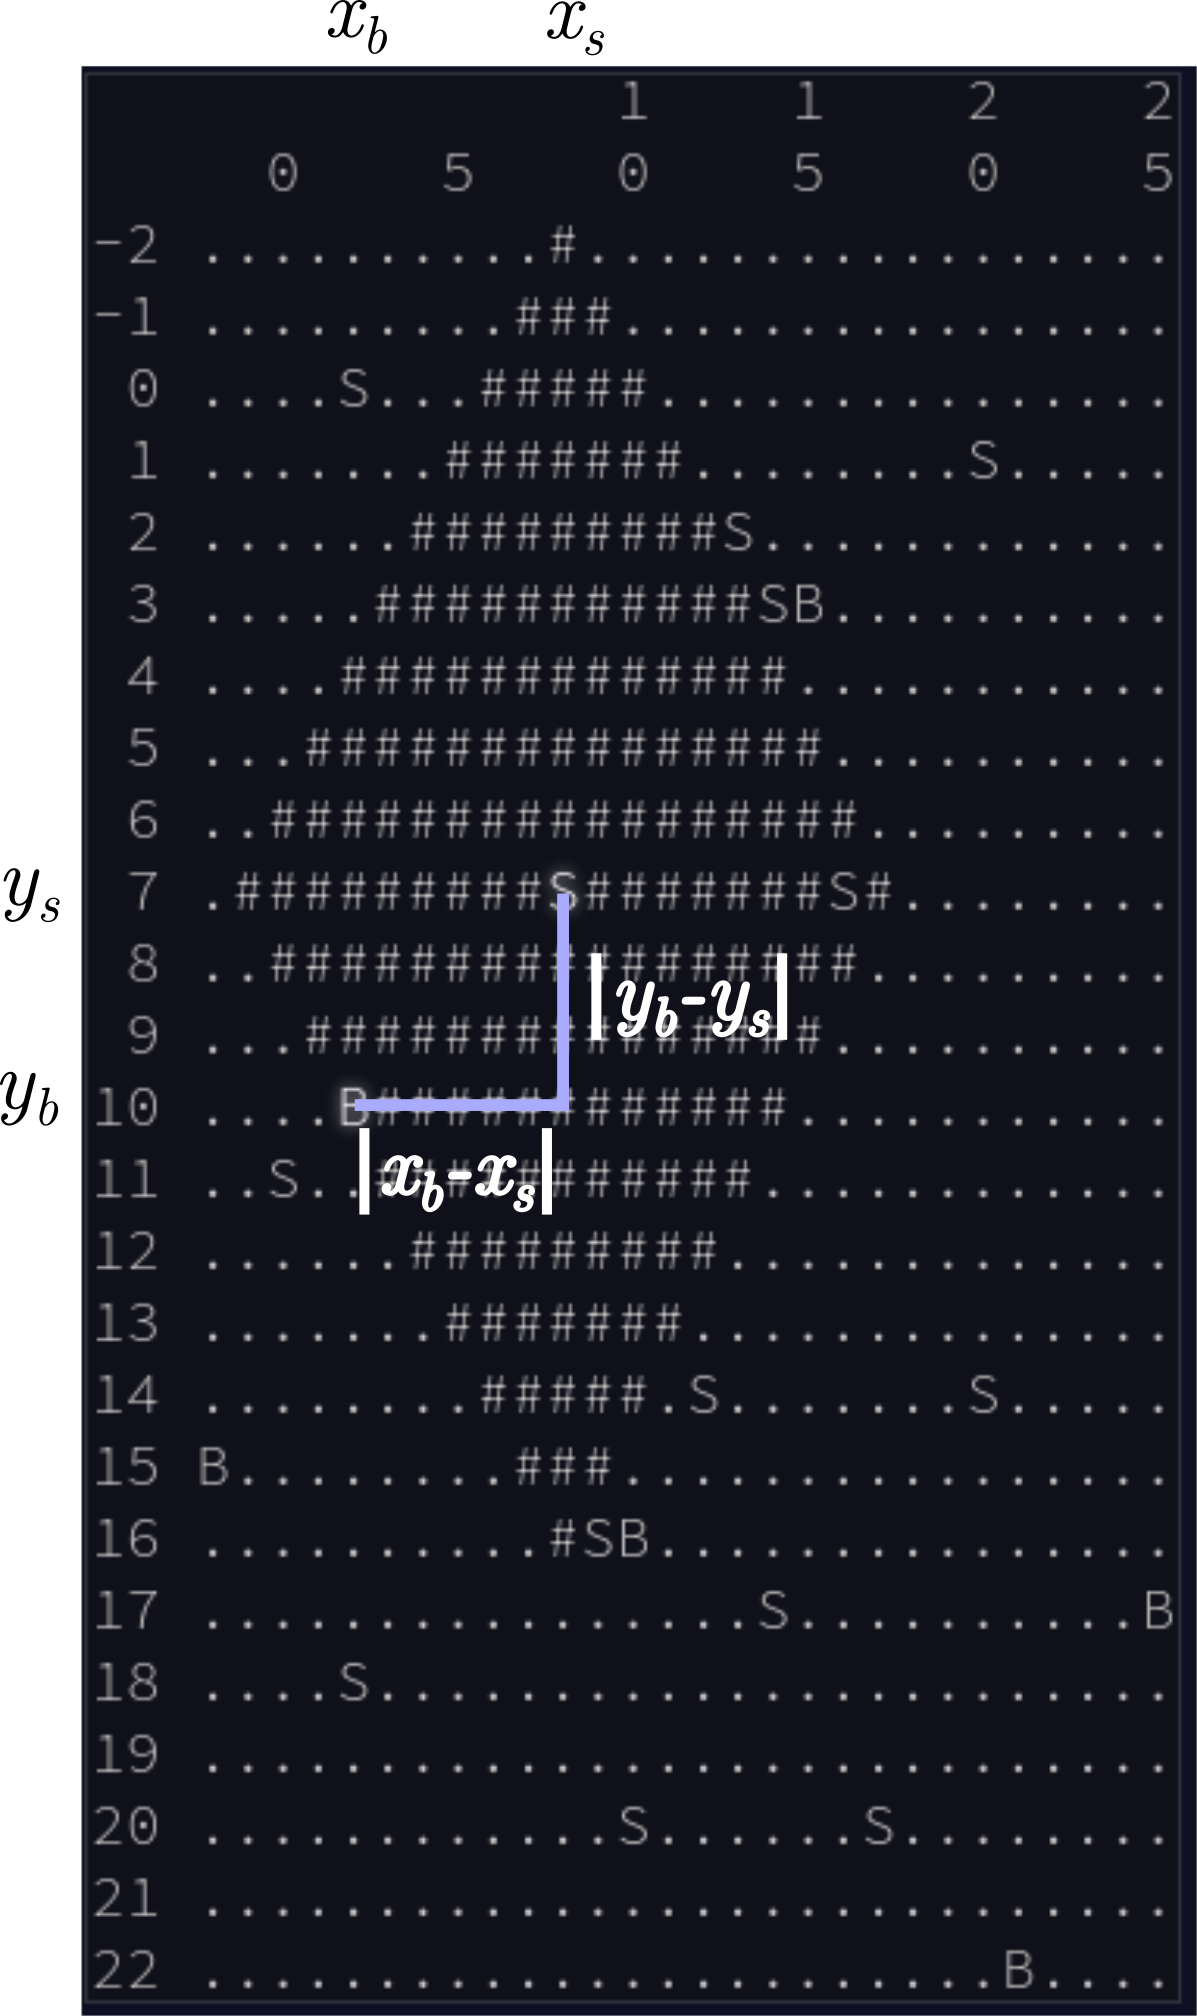
\includegraphics[width=0.8\textwidth]{illustration_coverage_radius.png}
                        \caption{Calculating the radius}
                    \end{figure}
                }
                \only<3->{
                    \begin{figure}
                        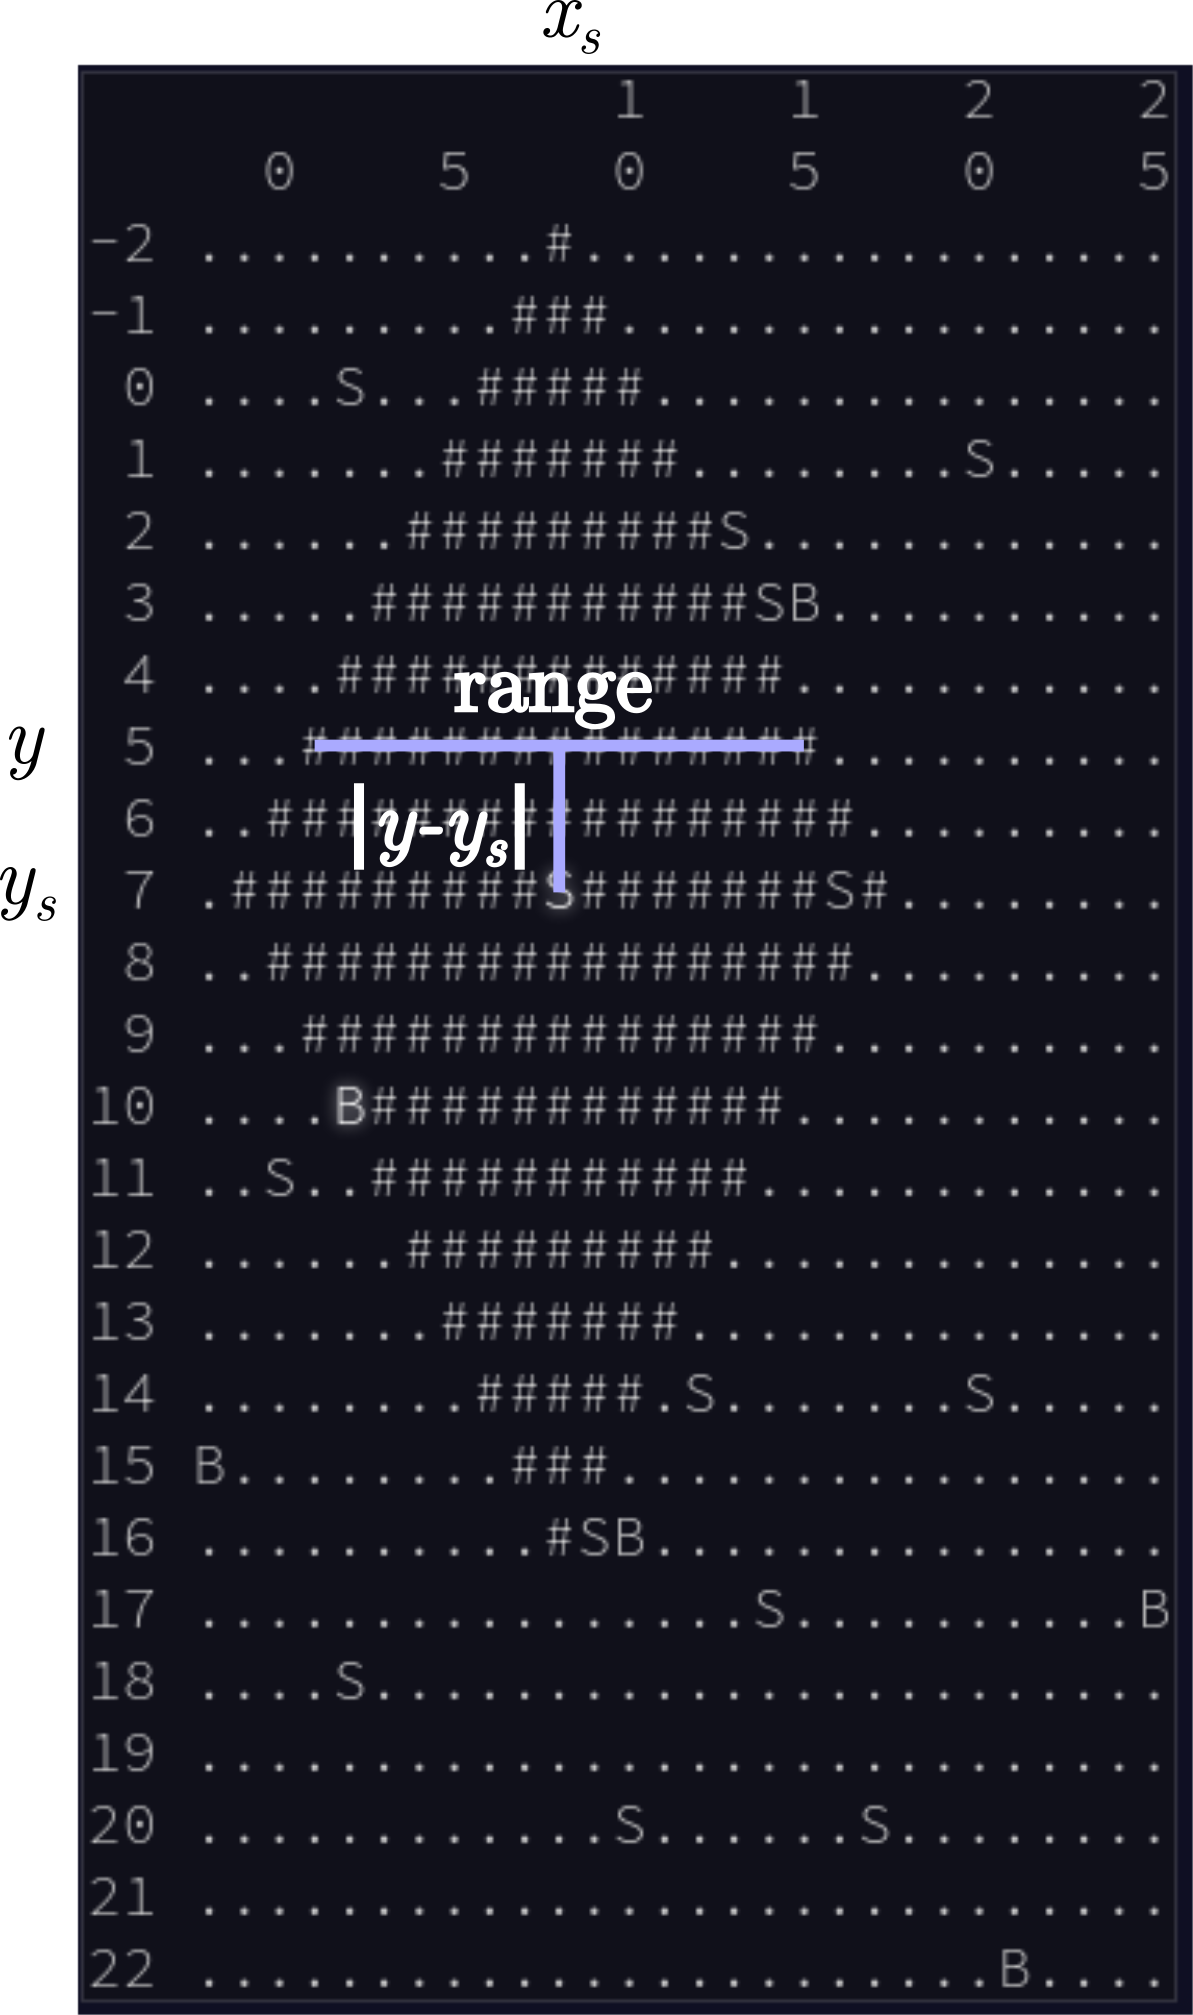
\includegraphics[width=0.8\textwidth]{illustration_coverage_range.png}
                        \caption{Calculating the range}
                    \end{figure}
                }
            \end{column}
        \end{columns}
    \end{frame}

    \begin{frame}[fragile]{The main problem with part b}
        How large would a 2D NumPy array of true/false values be?
        \pause
        \[
            4000000^2\cdot 1\,\mathrm{B} = \alert{15\,\mathrm{TB}}
        \]
        More if the datatype is not boolean:

        ~

        \begin{minted}[gobble=8, fontsize=\scriptsize]{python}
            >>> sys.getsizeof(np.zeros(10000000, dtype=bool))
            10000104

            >>> sys.getsizeof(np.zeros(10000000, dtype=int))
            80000104
        \end{minted}

        ~

        But a single row is only 4~MB!

    \end{frame}

    \begin{frame}{How about speed?}
    \end{frame}

    \begin{frame}{Big O notation}
    \end{frame}

    \begin{frame}{Big O notation}
        \begin{itemize}
            \item Number of sensors: $M=38$
            \item Number of grid points: $N=4000000^2=16\cdot 10^{12}$
        \end{itemize}
        Checking every sensor on every grid point:
        \[
            \mathcal O(MN)
        \]
        What if we can get rid of the grid points?
    \end{frame}

    \begin{frame}{An example}
        % \begin{align}
        %     x_1(y) = x_{11}
        %            + \frac{\overbrace{x_{12} - x_{11}}^{\Delta x_1}}
        %                   {\underbrace{y_{12}-y_{11}}_{\Delta y_1}}
        %              (y-y_{11})
        % \end{align}
        \begin{align*}
            x_1(y) = x_{11}
                   + \frac{\Delta x_1}{\Delta y_1}
                     (y-y_{11})
            \\
            x_2(y) = x_{21}
                   + \frac{\Delta x_2}{\Delta y_2}
                     (y-y_{21})
            \\
            \Delta x_1 = x_{12} - x_{11}
            ,\quad
            \Delta y_1 = y_{12} - y_{11}
            \\
            \Delta x_2 = x_{22} - x_{21}
            ,\quad
            \Delta y_2 = y_{22} - y_{21}
        \end{align*}
        \begin{align*}
            x_1(y) = x_2(y) \Rightarrow
            \\
            y = \frac{
                    y_{11} \Delta x_1 \Delta y_2 -
                    y_{21} \Delta x_2 \Delta y_1 +
                    (x_{21} - x_{11}) \Delta y_1 \Delta y_2
                }{
                    \Delta x_1 \Delta y_2 - \Delta x_2 \Delta y_1
                }
        \end{align*}
    \end{frame}

\end{document}
